\documentclass{article}
\usepackage{graphicx} 
\usepackage{hyperref}
\title{COP701 Sample Test cases}
\date{August 2024}
\begin{document}

\section{Introduction to IIT Delhi}
\subsection{Overview}
\subsubsection{History}

\textit{Indian Institute of Technology Delhi (IIT Delhi) is one of the premier engineering institutes in India.}
\textbf{Founded in 1961, IIT Delhi has grown into a world-class institution known for its cutting-edge research and academic excellence.}

\hrule

IIT Delhi is located in Hauz Khas, New Delhi. It offers undergraduate, postgraduate, and doctoral programs in various fields of engineering and technology.\par
The institute is renowned for its rigorous academic programs and distinguished faculty.

\begin{verbatim}
def iit_delhi_info():
    print("Welcome to IIT Delhi!")
    print("Explore the world-class research and academic programs.")
\end{verbatim}

For more information, visit the official IIT Delhi website: \href{https://www.iitd.ac.in}{IIT Delhi Official Website}

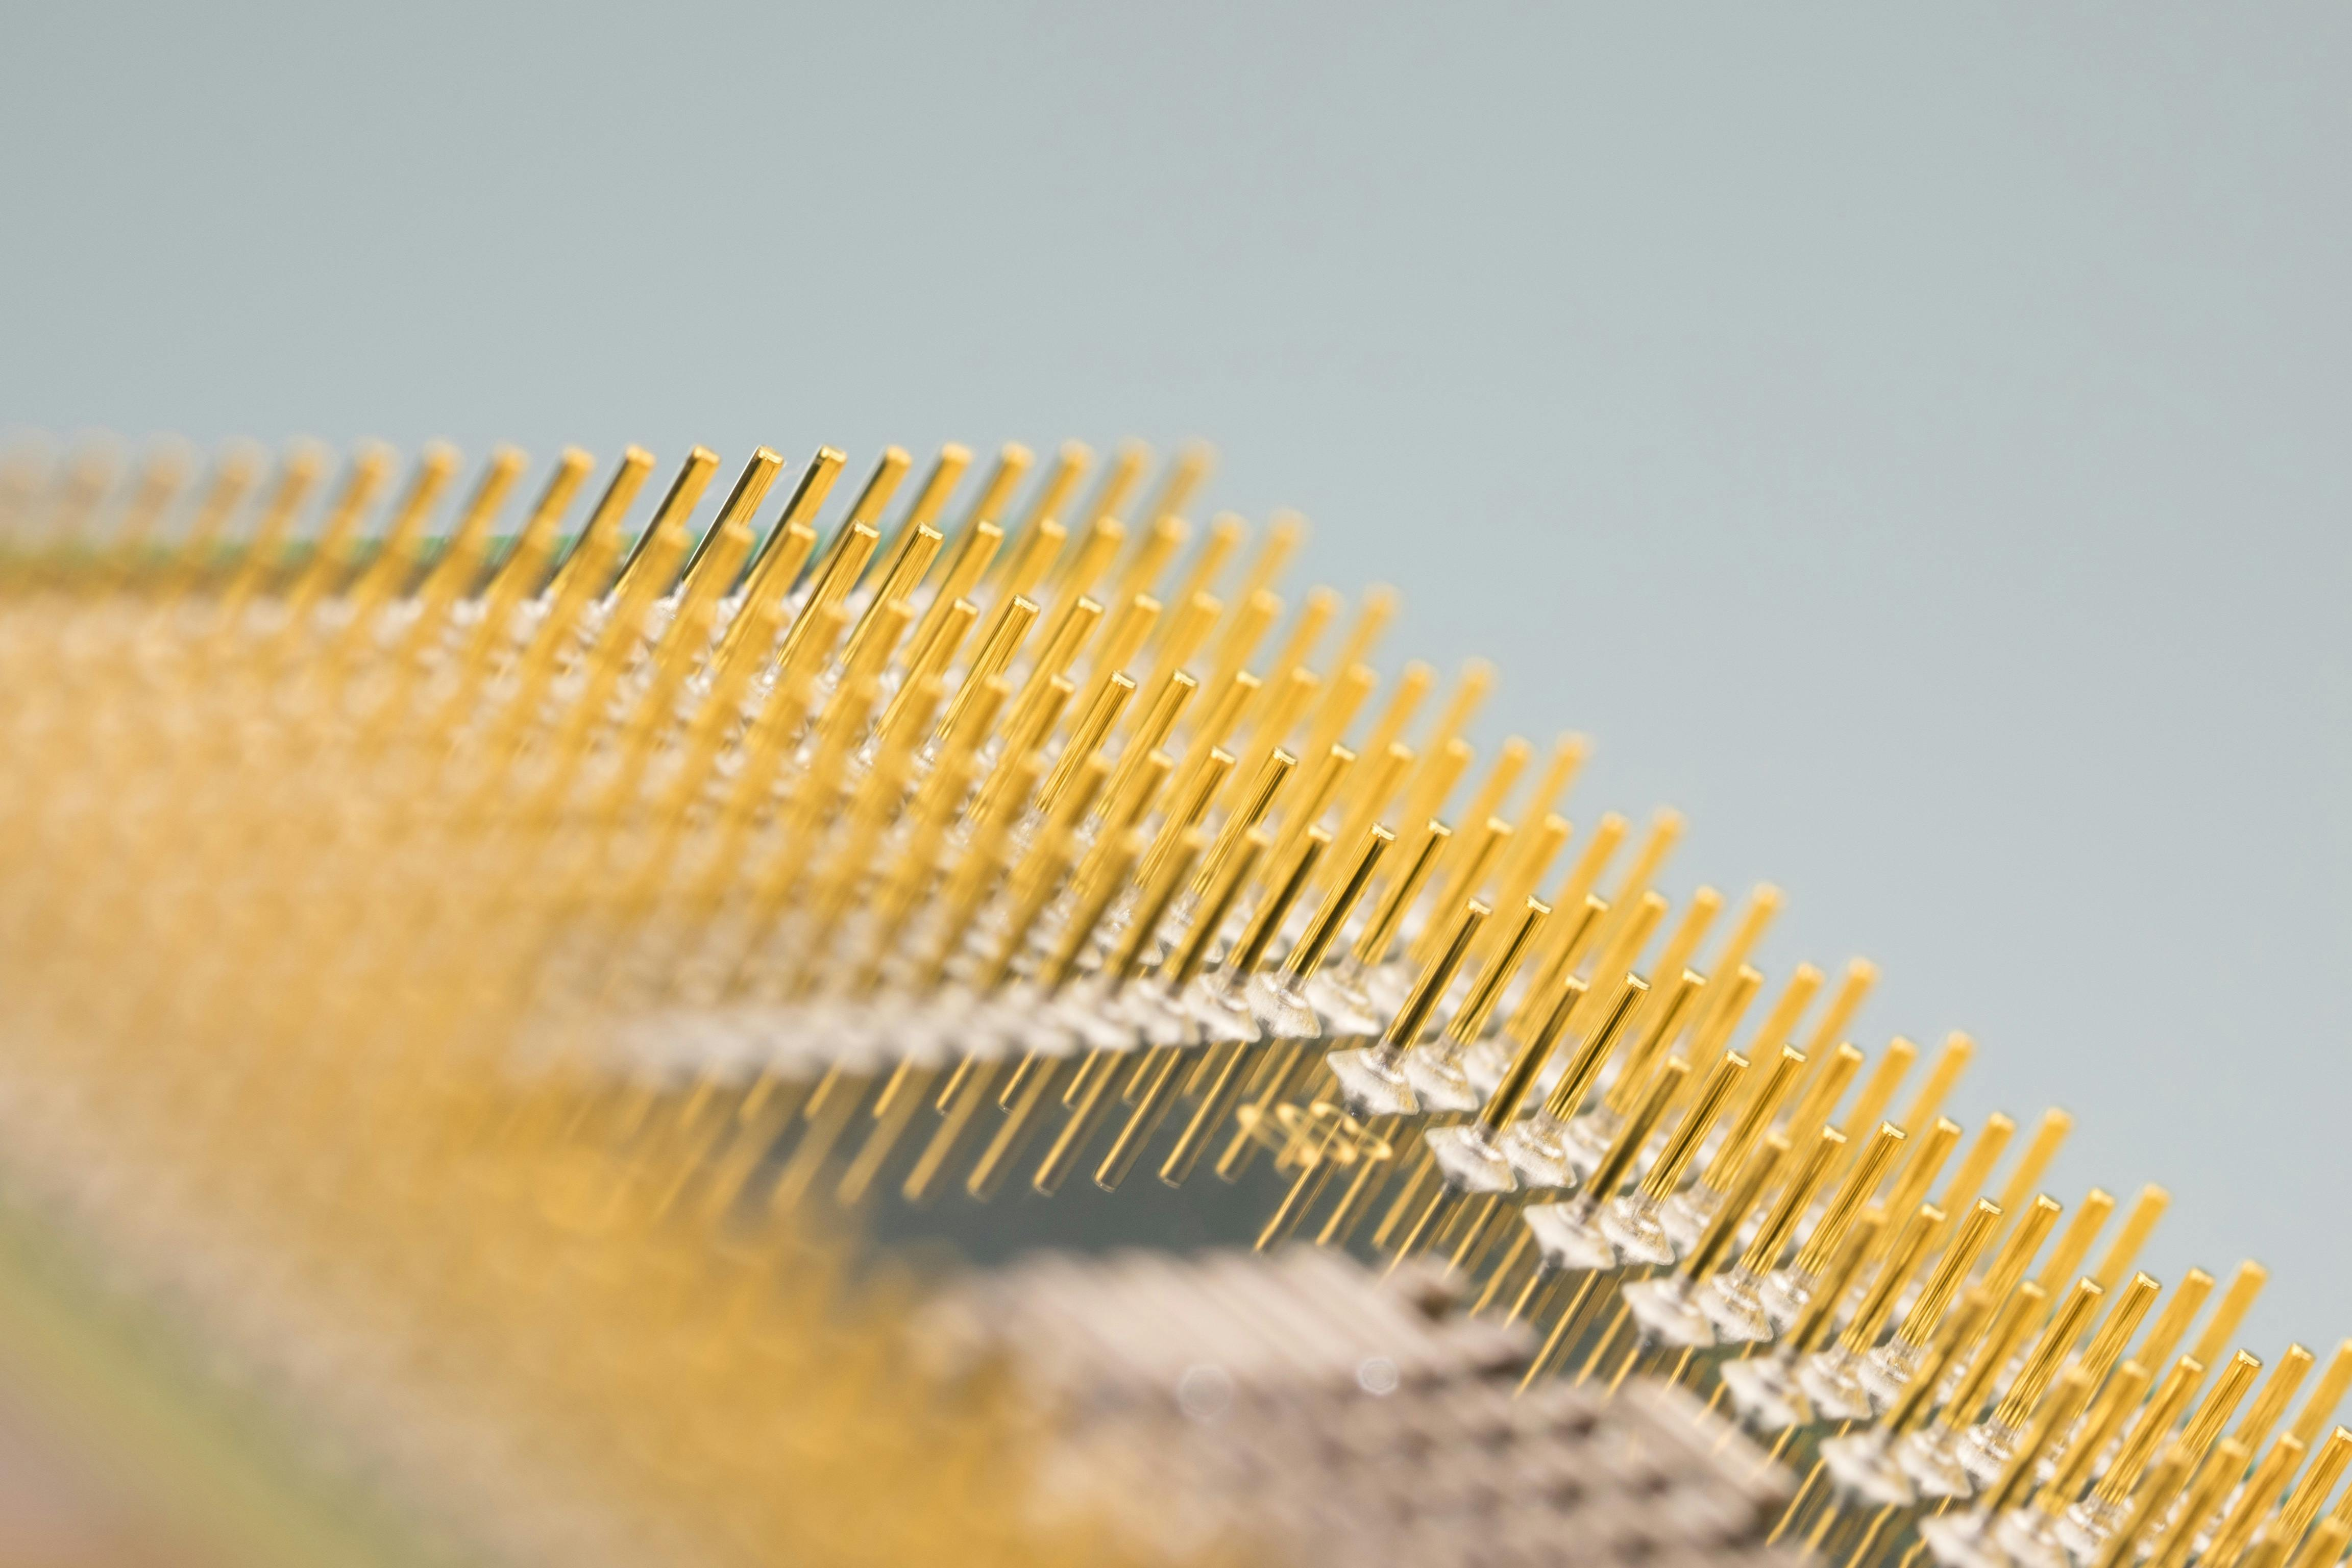
\includegraphics[width=0.5\textwidth]{TestCase/images/technology.jpg}

\begin{itemize}
    \item Established: 1961
    \item Location: Hauz Khas, New Delhi
    \item Programs: B.Tech, M.Tech, Ph.D., and more
\end{itemize}

\begin{enumerate}
    \item Campus Facilities
    \item Research Opportunities
    \item Alumni Achievements
\end{enumerate}

\begin{tabular}{|c|c|}
    \hline
    Department & Programs \\
    \hline
    Computer Science & B.Tech, M.Tech, Ph.D. \\
    Electrical Engineering & B.Tech, M.Tech, Ph.D. \\
    \hline
\end{tabular}

\end{document}